\documentclass{worksheetclass}

\usepackage{import}
\import{}{custom_macros.tex}

\title{The McKay Correspondence}

% DOCUMENT -----------------------------

\begin{document}

\maketitle

\tableofcontents

\section{Supersymmetric Yang-Mills theories}

    \subsection{Vacua space of SYM}

        Let us consider a supersymmetric gauge theory in $d=4$ with $k$ chiral sueprfields $\Phi_i$ ($i=1,\dots,k$) charged under the gauge group $G$ in an arbitrary representation $r_i$, in which the generators of $G$ are given by $T^a_{r_i}$ ($a=1,\dots,\dim G$). $\mathcal{W}_\alpha$ is the gaugina chiral superfield, containing the field strength. The lagrangian density on superspace is given by
        \begin{equation}
            \mathcal{L}=\int\d^2\theta\d^2\bar{\theta}~\Phi^\dagger e^{2V}\Phi+\int\d^2\theta\left\{\frac{\tau}{16\pi i}\tr(\mathcal{W}^\alpha\mathcal{W}_\alpha)+W(\Phi)\right\}+\text{c.c.}
        \end{equation}
        where we ignored the gauge indices. The superpotential $W(\Phi)$ is a holomorphic polynomial in the $\Phi_i$. The space of vacua is the space of configurations of $\Phi$ such that the $D$-terms and the $F$-terms vanish:
        \begin{subequations}
            \begin{empheq}[box=\widefbox]{align}
                D^a &\equiv \sum_i\Phi^\dagger_iT^a_{r_i}\Phi^i = 0,\\
                F^\dagger_i&\equiv \pdv{W}{\Phi^i}=0.
            \end{empheq}
        \end{subequations}
        In turns out that the full space of vacua of any supersymmetric gauge theory can be described as an algebraic variety.
    
    \subsection{$\mN=4$ super Yang-Mills theory in $D=4$}\label{sec:N4SCFT}

        \subsubsection{Superconformal group $\SU(2,2|4)$ and its representations}

            Conformal transformations and supersymmetries do not commute so the presence of conformal symmetry in addition to $\mN=4$ supersymmetry leads to an even larger group of symmetry known as the \emph{superconformal group}. In the $D=4,\mN=4$ case, the superconformal group is the super group\footnote{Supermanifold which is also a group with smooth product and inverse maps.} $\SU(2,2|4)$. The different component of the latter are
            \begin{itemize}
                \item \textbf{Conformal symmetries}: they form the 15-dimensional subgroup $\SO(2,4)$ and are generated by $P_\mu,M_{\mu\nu},K_\mu$ and $D$.
                \item \textbf{R-symmetry}: they form the 15-dimensional subgroup $\SO(6)_R$ and are generated by $T^A$ ($A=1,\dots,15$).
                \item \textbf{Poincaré supersymmetries}: they form the 16-dimensional sub group \todo{Why ?} and are generated by $Q^I_\alpha$ and $\bar{Q}^I_{\dalpha}$.
                \item \textbf{Conformal supersymmetries}: they form the 16-dimensional subgroup \todo{Why ?} and are generated by $S_{\alpha I}$ and $\bar{S}^{\dalpha I}$.
            \end{itemize}

            Conformal invariance of this theory can be seen as a consequence of the non-renormalization theorems.

        \subsubsection{Matter content}
            
            For $D=4,\mN=4$, there is only one kind of supermultiplet, the vector multiplet. Therefore, from an $\mN=4$ perspective, the only $\mN=4$ is a pure SYM. For extended supersymmetry, is is easier to express it in terms of $\mN=1$ superfield on $\mN=1$ superspace instead of looking to construct a superspace for $\mN=4$. In this case, we can see that the $\mN = 4$ vector superfield can be expressed in terms of $\mN = 1$ representations as one vector supermultiplet and three chiral scalar supermultiplets:
            \begin{equation}
                [\mN = 4 \text{ vector multiplet}] : V = (\lambda_\alpha, A_\mu, D) \oplus \Phi^A = (\phi^A,\psi^A_\alpha,F^A).
            \end{equation}
            with $A=1,2,3$ and
            \begin{align}
                \phi^A&=\phi^A_a T^a,\qquad \psi^A_\alpha=\psi^A_{\alpha,a}T^a,\qquad F^A=F^a_a T^a,\\
                \lambda^A&=\lambda^A_a T^a,\qquad A^A_\mu=A^A_{\mu,a}T^a,\qquad D^A=F^a_a T^a,\\
                V&=V_aT^a,\qquad \Phi^A=\Phi^A_aT^a,
            \end{align}
            where $T^a$ ($a=1,\dots,\dim G$) are the generators of $\mathfrak{g}$. The propagating degrees of freedom are therefore a vector field, three complex scalars and four gauginos. The Lagrangian is very much constrained by $\mN = 4$ supersymmetry. First, the chiral superfields $\Phi^A$ should transform in the adjoint representation of the gauge group $G$, since internal symmetries commute with supersymmetry. This means that all fields transform in the adjoint of $G$.
            
            Moreover, there is a large R-symmetry group\footnote{The fact that the scalar fields transform under the fundamental representation of $\SO(6)$, which is real, makes the R-symmetry group of the $\mN = 4$ theory being at most $\SU(4)$ and not $\U(4)$, in fact).}: $\SU(4)_R$. The four Weyl fermions transform in the fundamental of $\SU(4)_R$, while the six real scalars in the two times anti-symmetric representation, which is nothing but the fundamental representation of $\SO(6)$. The auxiliary fields are singlets under the R-symmetry group. Using $\mN = 1$ superfield formalism the Lagrangian reads
            \begin{align}
                \begin{split}
                    \L^{\mN=4}_{\text{SYM}} &= \frac{1}{32\pi}\Im \left(\tau\int\d^4x\tr(W^\alpha W_\alpha)\right)+\int\d^2\theta\d^2\bar{\theta}\tr\sum^3_{A=1}\bar{\Phi}^Ae^{2gV}\Phi^A\\
                    &\quad-\int\d^2\theta\sqrt{2g}\tr\Phi_1[\Phi_2,\Phi_3]+\text{h.c.}
                \end{split}\label{eq:N4lag}
            \end{align}
            where as usual $W_\alpha=-\frac{1}{4}\bar{D}\bar{D}(e^{-V}D_\alpha e^V)$ is the gaugino superfield. This lagrangian is indeed invariant under the superPoincaré algebra and under the gauge transformations
            \begin{align}
                e^V &\to e^{i\bar{\Lambda}} e^V e^{-i\Lambda} \text{ (which implies that $W_\alpha \to e^{i\Lambda}W_\alpha e^{-i\Lambda}$)},\\
                \Phi^A &\to e^{i\Lambda}\Phi^A.
            \end{align}
            The large $\SU(4)_R$ R-symmetry group forbids of having a superpotential. The commutator in the third term of \eqref{eq:N4lag} appears for the same reason as for the $\mN = 2$ Lagrangian. Notice that the choice of a single $\mN = 1$ supersymmetry generator breaks the full $\SU(4)_R$ R-symmetry to $\SU(3)\times \U(1)_R$. The three chiral superfields transform in the $\boldsymbol{3}$ of $\SU(3)$ and have R-charge $R = 2/3$ under the $\U(1)_R$. It is an easy but tedious exercise to perform the integration in superspace and get an explicit expression in terms of fields. Finally, one can solve for the auxiliary fields and get an expression where only propagating degrees of freedom are present, and where $\SU(4)_R$ invariance is manifest.

            \begin{figure}[H]
                \centering
                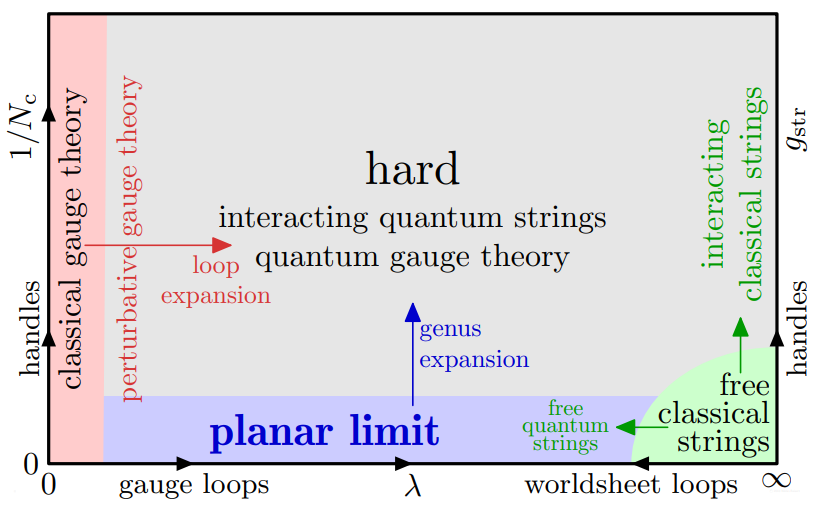
\includegraphics[scale=0.4]{Pictures/N4SYMparameterspace.png}
                \caption{Map of the parameter space of $\mN=4$ SYM or strings on $\text{AdS}_5\times S^5$, from \cite{Beisert_2011}.}
            \end{figure}
            \todo{Explain this diagram.}

        \subsubsection{Moduli space and dynamical phases}

            The scalar potential in \eqref{eq:N4lag} can be written in a rather compact form in terms of the six real scalars $X^i$ making up the three complex scalars $\phi^A$ and reads
            \begin{equation}
                V(X_1,\dots,X_6) = \frac{1}{2}g^2\tr\sum^6_{i,j=1}[X_i,X_j]^2.
            \end{equation}
            The positive definite behavior of the Cartan-Killing form on the compact gauge algebra $\g$ implies that each term in the sum is positive or zero. In other words, $V=0$ is equivalent to
            \begin{equation}
                [X^i,X^j]=0,\qquad i,j=1,\dots,6.
            \end{equation}
            This means that the potential vanishes whenever the scalar fields belong to the Cartan subalgebra of the gauge group $G$. At a generic point of the moduli space, the gauge group is broken to $\U(1)^r$ where $r$ is the rank of $\mathfrak{g}$.
            This equations admit two classes of solutions:
            \begin{itemize}
                \item $\langle X^i\rangle=0$ for all $i=1,\dots,6$. This is the \emph{superconformal phase}. Neither the gauge symmetry nor the superconformal symmetry is broken. The physical states and operators are gauge invariant and transform under
                unitary representations of $\SU(2,2|4)$.
                \item  $\langle X^i\rangle\neq0$ for at least one $i$. This is the \emph{spontaneously broken Coulomb phase}. The gauge algebra $\g$ is going to be broken to $\U(1)^r$, where $r\equiv\rank\g$. The low energy behavior is then the one of $r$ copies of $\mN=4$ $\U(1)$ gauge theories. Superconformal symmetry is spontaneously broken since the non-zero VEV $\langle X^i\rangle$ sets a scale.
            \end{itemize}

            \begin{result}
                \textbf{$\boldsymbol{\mN=4}$ Yang-Mills theory.} There is only one $D=4,\mN=4$ Yang-Mills theory and it contains $3$ $\mN=1$ chiral scalar supermutliplet and $1$ $\mN=1$ vector supermultiplet (up to $g$ and $\tau$). This theory is conformal and can be recovered from dimensional reduction of $D=10,\mN=1$ Yang-Mills on $\mathbb{T}^6$.
            \end{result}
        
    \subsection{Gauge anomaly}\label{sec:anomalies}
        
        The \emph{anomaly degree} $A(\rho)$ of a representation $\rho$ is defined as
        \begin{equation}
            \frac{1}{2}\tr(T_a\{T_b,T_c\})=A(\rho)d_{abc}
        \end{equation}
        where $d_{abc}$ is an invariant symmetric tensor of the Lie algebra of $G$, independent of the representation. One can show that $A(\rho^*)=-A(\rho)$ so self dual representation have $A(\rho)=0$ in particular. The only simple Lie groups that allow for a complex non-self-conjugate representation are $\SU(n)$ with $n\geq3$. We can normalize $d_{abc}$ such that $A(\rho)=1$ for the fundamental $n$-dimensional representations.

\printbibliography

\end{document}